\documentclass[conference]{IEEEtran}
\usepackage{amsmath,amsfonts}
\usepackage{algorithmic}
\usepackage{algorithm}
\usepackage{array}
\usepackage[caption=false,font=normalsize,labelfont=sf,textfont=sf]{subfig}
\usepackage{textcomp}
\usepackage{stfloats}
\usepackage{url}
\usepackage{verbatim}
\usepackage{graphicx}
\usepackage{cite}
\usepackage[hypcap=false]{caption}
\usepackage{float}

% Set path for images
\graphicspath{ {./images/} }

\newenvironment{Figure}
    {\par\medskip\noindent\minipage{\linewidth}}
    {\endminipage\par\medskip}


\begin{document}

\title{Explainable Machine Learning Guided Modeling for Antennas\\
}

\author{\IEEEauthorblockN{Tyler Carr}
\IEEEauthorblockA{\textit{WiDE Laboratory} \\
\textit{Embry-Riddle Aeronautical University}\\
Daytona Beach, Florida\\
carrt12@my.erau.edu}
\and
\IEEEauthorblockN{Cameron Martinez}
\IEEEauthorblockA{\textit{WiDE Laboratory} \\
\textit{Embry-Riddle Aeronautical University}\\
Daytona Beach, Florida \\
martc114@my.erau.edu}
\and
\IEEEauthorblockN{Dr. Eduardo Rojas-Nastrucci}
\IEEEauthorblockA{\textit{WiDE Laboratory} \\
\textit{Embry-Riddle Aeronautical University}\\
Daytona Beach, Florida \\
rojase1@erau.edu}
\and
\IEEEauthorblockN{Dr. M. Ilhan Akbas}
\IEEEauthorblockA{\textit{WiDE Laboratory} \\
\textit{Embry-Riddle Aeronautical University}\\
Daytona Beach, Florida \\
akbasm@erau.edu}
}

\maketitle

\begin{abstract}
    Antenna design processes require extensive electromagnetic (EM) simulation tasks that are resource-intensive, time-consuming, and prone to interruptions. Design equations are only available for predefined and limited antenna geometries. By applying a machine learning (ML) model to a limited set of data from electromagnetic simulations of a leaky wave antenna, performance metrics can be predicted significantly quicker than running simulations for an extensive range of geometric variations. Insights about which geometric parameter had the most significant impact on the prediction can be drawn from the model – hence, explainable ML - and included in the output. The model can be used for inverse design techniques, where the performance requirements are provided as input, and the model generates a geometric solution that meets those requirements. Explainable ML processes can then be applied to analyze which geometric parameter had the largest impact on the performance prediction. The design process was tested on XXX.
\end{abstract}

\section{Introduction}
In the realm of wireless communication, microstrip patch antennas have emerged as a favored choice due to their compact size, ease of fabrication, and adaptability to various applications. Comprised of a metallic patch on a dielectric substrate, these antennas offer tunable performance characteristics such as resonant frequency, bandwidth, and radiation pattern. Despite their simplicity, predicting the behavior of microstrip patch antennas involves intricate considerations of parameters like patch dimensions, substrate properties, and feeding mechanisms \cite{Patch_antennas}.

The basic design of this work is a inset-fed microstrip patch antenna, similar to that shown in \cite{inset_feed_pa}. It uses Rogers RT/duroid 5870, with a dielectric constant of 2.33 and dissipation factor of 0.001, for the dielectric substrate layer. There are a few crucial design parameters for the microstrip patch antenna, which are outlined in Figures~\ref{Planar view} and~\ref{3D view}. This design is implemented into ANSYS High-Frequency Structure Simulator (HFSS) so that it can be modeled and simulated. 

\begin{Figure}
    \centering
    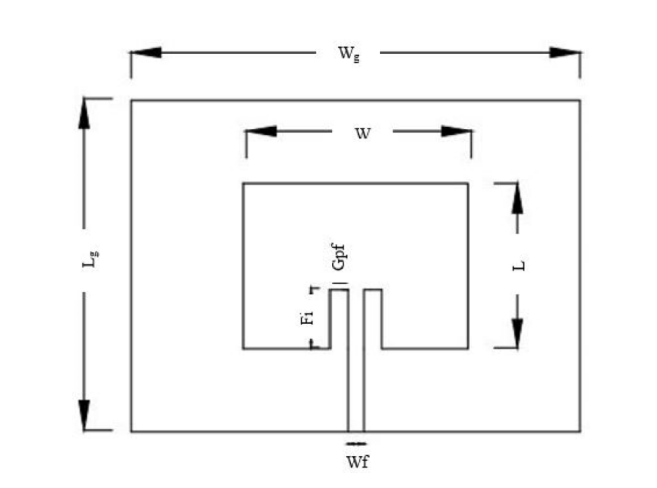
\includegraphics[width=3in]{inset_fed patch antenna.png}
    \captionof{figure}{Planar view of inset-fed patch antenna}
    \label{Planar view}
\end{Figure}


\begin{Figure}
    \centering
    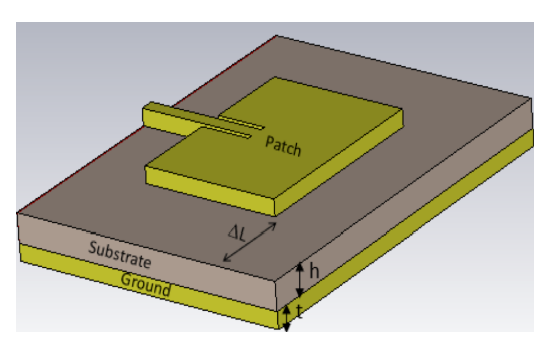
\includegraphics[width=3in]{3D patch antenna.png}
    \captionof{figure}{3-D view of inset-fed patch antenna }
    \label{3D view}
\end{Figure}

\textlangle ~insert intro about leaky wave antenna\textrangle

Traditionally, the design and analysis of microstrip patch antennas and leaky wave antennas relied on theoretical models and electromagnetic simulation software, like HFSS, which necessitates significant computational resources and manual iterations~\cite{john_antenna_2009,ranjan_design_2023,liu_efficient_2014}. However, the integration of machine learning (ML) techniques has revolutionized this process by enabling rapid prediction and optimization of antenna behavior. By leveraging datasets of simulated antenna configurations, ML models can learn complex patterns and relationships, thus streamlining antenna development and enhancing performance in wireless communication systems.

One important way to evaluate antenna performance is through its scattering parameters (S-parameters), specifically its $S_{11}$. This is known as the reflection coefficient or return loss, and represents the ratio of input power to reflected power, typically expressed in decibels (dB). For passive systems, this value is always negative. A return loss of less than -10dB demonstrates a high level of impedance matching for an antenna, and is crucial for optimizing antenna performance in terms of signal strength, bandwidth, and radiation efficiency. 

By changing the main antenna design parameters, a new geometry is created, which generates a new $S_{11}$ response. These geometry specific $S_{11}$ values, along with the parameters of that geometry, were compiled into a dataset, which was then used for training and validating the machine learning model. Both the patch antenna and the leaky wave antenna were put through this process, the first of which was used to prove that the process works well with a simple antenna design and the latter to test the method on a more advanced antenna design. The dataset of the patch antenna consists of 40,905 rows, which was comprised of 405 unique geometries with $S_{11}$ values simulated across 101 frequency range values between 4GHz and 12GHz. Similarly, the dataset of the leaky wave antenna consists of 23,735 rows, which was comprised of 233 unique geometries with $S_{11}$ values simulated across 101 frequency range values between 11GHz and 20GHz. Tables~\ref{antenna_dataset_p} and~\ref{antenna_design_lw} describes the relationship between the data.


\begin{table}[h]
\caption{Patch Antenna Dataset}
\begin{center}
\begin{tabular}{ |l|l|l|l| }
    \hline
    Parameter & Min & Max & Step \\ 
    \hline
    inset\_dist [mm] & 0.6 & 1.4 & 0.4 \\
    \hline
    L [mm] & 11.5 & 12.5 & 0.5 \\
    \hline
    sub\_thick [mm] & 2 & 2 & N/A \\
    \hline
    W [mm] & 14.0 & 15.6 & 0.8 \\
    \hline
    W0 [mm] & 2.5 & 3.5 & 0.5 \\
    \hline
    y0 [mm] & 3.0 & 5.0 & 0.5 \\
    \hline
    Freq [GHz] & 4.0 & 12.0 & 0.08 \\
    \hline
\end{tabular}
\end{center}
\label{antenna_dataset_p}
\end{table}


\begin{table}[h]
\caption{Leaky Wave Antenna Dataset}
\begin{center}
\begin{tabular}{ |l|l|l|l| }
    \hline
    Parameter & Min & Max & Step \\ 
    \hline
    cpw\_in [mm] & 1.5 & 2.5 & 0.25 \\
    \hline
    feed\_l [mm] & 3.25 & 4.25 & 0.25 \\
    \hline
    patch\_l [mm] & 3.25 & 4.25 & 0.25 \\
    \hline
    cpw\_g [mm] & 0.12 & 0.36 & 0.06 \\
    \hline
    Feed\_W [mm] & 0.5 & 2.0 & 0.5 \\
    \hline
    ground\_w [mm] & 0.5 & 1.5 & 0.5 \\
    \hline
    patch\_ground\_w [mm] & 0.5 & 1.5 & 0.5 \\
    \hline
    patch\_w [mm] & 4.5 & 5.0 & 0.25 \\
    \hline
    Freq [GHz] & 11.0 & 20.0 & 0.09 \\
    \hline
\end{tabular}
\end{center}
\label{antenna_design_lw}
\end{table}


\section{Methodology}
Making up the generated dataset that will be searched to find the optimal antenna geometry are all possible combinations of geometries and frequencies. This added up to a total of 9,720 unique geometries for the patch antenna and 327,892 for the leaky wave antenna. The simulated $S_{11}$ values for each antenna were used for the original simulated values since they were already given, and predictions were generated for the rest of the geometry and frequency combinations. This new dataset added up to a total of 981,720 and 33,117,092 rows for the patch antenna and leaky wave antennas, respectively.

In order to determine the optimal antenna geometry, a machine learning model was employed. This model was trained with a supervised learning method using the dataset of simulated data for the leaky wave antenna. This is the model that will be used to make predictions in the simulated dataset.

The generated dataset with predictions can be searched by specifying the desired $S_{11}$ value and a frequency range that the antenna should operate within. Antenna geometries that match the search are returned, which saves significant time that would be required to set up and perform additional simulations. When seeking an optimal geometry between a certain frequency range, the geometries that results in the $S_{11}$ with the lowest maximum $S_{11}$ range would be chosen.


\subsection{Metrics}
In order to determine if a $S_{11}$ value was predicted accurately or not, a tolerance was utilized. The tolerance is the maximum deviation from the true value that is allowed, and the prediction is considered accurate if it is within the tolerance. This concept is used when calculating the score of a model~\eqref{eq:tolerance}, with $\epsilon$ being tolerance, $\hat{y_i}$ being the $i$th $S_{11}$ prediction, $y_i$ being the $i$th true $S_{11}$ value, and $n$ being the count of data points. The tolerance is assumed to be one when calculating all scores.

Two other common metrics to compare algorithm performance in addition to the tolerance mentioned above are the $R^2$ score~\eqref{eq:rsquared} and the Root Mean Squared Error (RMSE)~\eqref{eq:rmse}~\cite{shcherbakov_survey_2013}. The $R^2$ score represents how well the regression line fit to the data, and the RMSE represents the difference between the predicted and true values.

\begin{figure}[h]
    \begin{equation}
        \text{Score} = \frac{1}{n} \sum_{i=1}^{n}(\left|\hat{y_i} - y_i\right| \leq \epsilon)
        \label{eq:tolerance}
    \end{equation}
    \begin{equation}
        R^2 = 1 - \frac{\sum_{i}(\hat{y_i} - \bar{y})^2}{\sum_{i}(y_i - \bar{y})^2}
        \label{eq:rsquared}
    \end{equation}
    \begin{equation}
        {RMSE} = \sqrt(\frac{1}{n} \sum_{i=1}^{n}(y_i - \hat{y}_i)^2)
        \label{eq:rmse}
    \end{equation}
    \caption{Evaluation Metrics}
\end{figure}



\subsection{Preprocessing}
Preprocessing needed to be performed on the data features before using them with any model. Firstly, the dataset was split into training and testing sets, with 20\% being reserved for testing and comparing the performance of the models, and the remaining 80\% used to train the models. A standardized scaler was then used to standardize the geometries and frequencies by removing the mean and dividing each value by the standard deviation. This is to ensure the values all have the same scale to improve model performance~\cite{9119820}. 


\subsection{Comparing Models}
Two different libraries were compared in order to determine the best model for this type of dataset. The first library that was used is TensorFlow, which was used to create a DNN (deep neural network)~\cite{tensorflow2015-whitepaper}. The performance of the DNN was compared to many of Scikit-learn's regression models~\cite{scikit-learn}.

To keep the comparison between the algorithms fair, all preprocessing steps were performed in the same way when comparing the performance of different libraries and algorithms. When splitting the dataset into training and testing portions, the dataset was split with the same random state, meaning that every model received the same random subset of data for training. Additionally, the models were evaluated in the same way using the same performance metrics between the different libraries. All of the following were performed on the same machine to eliminate the possibility of hardware anomalies. The machine that was used contained an Intel i9-10900X 3.70 GHz CPU with 64 GB RAM and a NVIDIA GeForce RTX 3090 graphics card. 


\subsection{TensorFlow}
TensorFlow was used to create a DNN (deep neural network), which is useful for large datasets. The main benefit of a DNN is that it automatically figures out the most important correlations between features for you. 

The hyperparameters of the DNN were tuned in an attempt to both improve the accuracy and reduce the error rate of the model. This was done by adjusting various hyperparameters of the model, including the number of layers in the network, the rate at which the model learns, and the unit of each layer, which represents the number of neurons and outputs. This was done using a randomized searching method provided by Keras Tuner~\cite{omalley2019kerastuner}. In typical grid search hyperparameter tuning, the search space grows too large to be feasibly tested fairly quickly. With the randomized search method, a random subset of hyperparameter combinations can be tested. The most optimal results are not guaranteed, but it can get relatively close~\cite{meanti_efficient_2022}. 


\subsection{Scikit-learn}
Scikit-learn is another popular machine learning library where the typical use case is smaller datasets with feature extraction already having been performed. There are a multitude of regression models provided by Scikit-learn. The models that were analyzed in this test were RandomForestRegressor, GradientBoostingRegressor, AdaBoostRegressor, CatBoostRegressor, XGBRegressor, and DecisionTreeRegressor.

Similarly to with TensorFlow, a randomized search was used to determine the best hyperparameters for each model's use case. Once the optimization was performed, all of the best models had their performance compared using the same metrics. 

\subsection{Model Performance Analysis}
A manual analysis was performed using a number of random unique antenna geometry configurations for both antenna designs. The geometries selected have never been seen by the simulation, training set, or testing set. They then have both their simulated and predicted $S_{11}$ values for the entire frequency range from the HFSS and best chosen model compared. This process is done in order to narrow in on random samples of actual data to check that the model is performing comparably to the simulation software. The geometric parameters of the chosen unseen geometries are recorded in Table~\ref{unseen_geometries_p} and Table~\ref{unseen_geometries_lw}.

\begin{table}[h]
\caption{Unseen Geometry Parameters}
\begin{center}
\begin{tabular}{ |l|l|l|l|l|l|l| }
    \hline
    ID & 1 & 2 & 3 & 4 & 5 & 6 \\ 
    \hline
    inset\_dist [mm] & 0.6 & 0.6 & 1.0 & 1.4 & 1.4 & 1.4 \\
    \hline
    L [mm] & 11.5 & 12.0 & 12.0 & 11.5 & 11.5 & 11.75 \\
    \hline
    sub\_thick [mm]  & 2.0 & 2.0 & 2.0 & 2.0 & 2.0 & 2.0 \\
    \hline
    W [mm]  & 14.8 & 14.8 & 15.6 & 15.6 & 15.4 & 15.4 \\
    \hline
    W0 [mm] & 2.5 & 2.75 & 3.5 & 3.5 & 3.5 & 3.5 \\
    \hline
    y0 [mm] & 4.25 & 4.5 & 4.25 & 4.25 & 4.5 & 4.75 \\
    \hline
\end{tabular}
\end{center}
\label{unseen_geometries_p}
\end{table}    

\begin{table}[h]
\caption{Unseen Geometry Parameters}
\begin{center}
\begin{tabular}{ |l|l|l|l|l|l|l| }
    \hline
    ID & 1 & 2 & 3 & 4 & 5 & 6 \\
    \hline
    cpw\_in [mm] & 2.5 & 1.75 & 1.75 & 1.75 & 2.5 & 2.5 \\
    \hline
    feed\_l [mm] & 3.25 & 3.25 & 3.5 & 4 & 3.75 & 4 \\
    \hline
    patch\_l [mm] & 3.5 & 3.25 & 3.5 & 4 & 3.75 & 4.25 \\
    \hline
    cpw\_g [mm] & 0.18 & 0.3 & 0.3 & 0.12 & 0.36 & 0.24 \\
    \hline
    Feed\_W [mm] & 1.25 & 0.5 & 1.25 & 1.25 & 0.5 & 1.75 \\
    \hline
    ground\_w [mm] & 0.5 & 0.75 & 1 & 1.25 & 1.5 & 1 \\
    \hline
    patch\_ground\_w [mm] & 0.5 & 1 & 0.5 & 1.5 & 1 & 1.25 \\
    \hline
    patch\_w [mm] & 5 & 5 & 5 & 4.75 & 5 & 4.5 \\
    \hline
\end{tabular}
\end{center}
\label{unseen_geometries_lw}
\end{table}    
    

\subsection{Finding Optimal Geometry}
The flowchart in Figure~\ref{data_flow} gives a visual representation of how the data flows through the algorithm. All of the steps up until generating predictions are performed initially for any new antenna configuration that the model hasn't seen yet. The last few steps, starting at filtering rows, are performed every time a new optimal geometry is searched using a specified $S_{11}$ and frequency range. 

\begin{Figure}
\centering
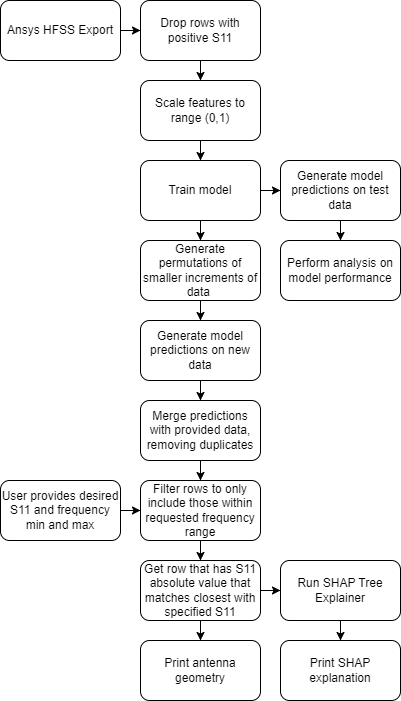
\includegraphics[width=3.0in]{methodology}
\captionof{figure}{Flow of data through the system}
\label{data_flow}
\end{Figure}

A GUI (graphical user interface) was created in order to make the process of filtering optimal geometries more intuitive. The GUI include an input area, where a user can input a desired $S_{11}$ and frequency range. Once these are entered, all of the permutations are filtered and the best performing optimal geometries are shown. A graph of frequency and predicted $S_{11}$ is also shown, where each optimal geometry is plotted. The desired $S_{11}$ and frequency range are also represented on the graph so it's clear what area of the graph is being focused on.


\section{Results}
\subsection{Library and Model Comparison with the Patch Antenna}
Both antennas were used to test and compare the performance of models from the two different libraries: TensorFlow and Scikit-learn. The best performing model was chosen from each library, and their training time, predicting time, accuracy, and RMSE were compared in order to select the best model.

The Keras Tuner search for optimal hyperparameters of the DNN provided the results in Table~\ref{keras_best_params}. This was tested for both the patch antenna and the leaky wave antenna. The patch antenna was found to work best with a smaller DNN consisting of two layers, where the leaky wave antenna performed best with only one. The optimal learning rate was similar for both antennas, with the patch antenna having the higher learning rate. The DNNs were able to predict $S_{11}$ values with an error tolerance of~$\pm$1dB for the patch antenna and leaky wave antenna with a 84.17\% and 27.26\% accuracy respectively. These accuracies are not desirable, and might be an indicator that a DNN is too complex for this job.

\begin{table}[h]
\caption{Keras Tuner Best Hyperparameters}
\begin{center}
\begin{tabular}{ |l|l|l|l| }
    \hline
    Name & Patch Value & Leaky Wave Value \\ 
    \hline
    num\_layers & 2 & 1 \\  
    \hline
    units\_0 & 256 & 224 \\
    \hline
    units\_1 & 32 & N/A \\
    \hline
    learning\_rate & 0.0841 & 0.0522 \\
    \hline
\end{tabular}
\end{center}
\label{keras_best_params}
\end{table}

Figure~\ref{dnn_loss_graph} shows how the DNN's loss decreased as the number of epochs increased for both the patch antenna and the leaky wave antenna. The loss was significantly less for the patch antenna, which is to be expected as the model is having an easier time fitting to the simpler antenna design. The fact that this graph shows both the training and testing decreasing shows that the model is converging. Additionally, the model is not overfitting. 

\begin{Figure}
    \centering
    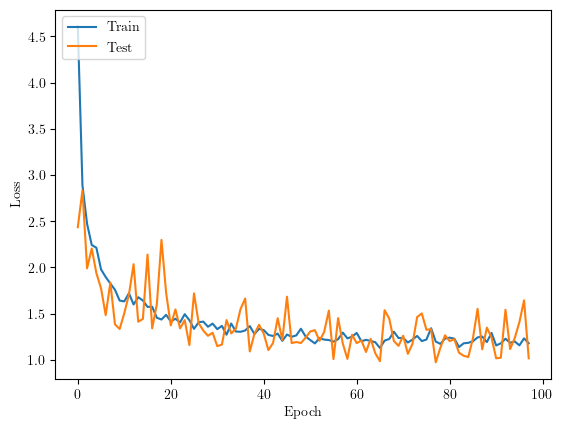
\includegraphics[width=3in]{loss}
    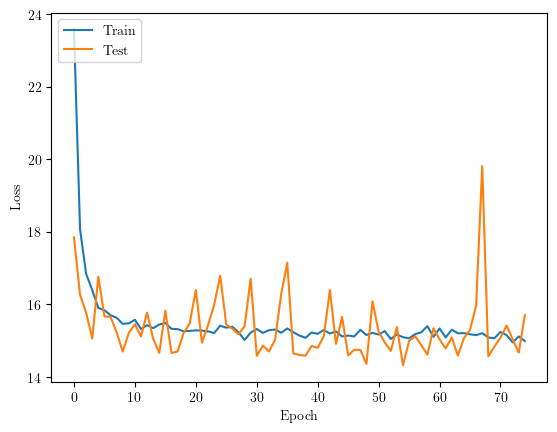
\includegraphics[width=3in]{loss_lw}
    \captionof{figure}{DNN Loss Graph for Patch and Leaky Wave Antennas}
    \label{dnn_loss_graph}
\end{Figure}

Each of the Scikit-learn regression models performed differently than one another. After performing a randomized search for the best hyperparameters for each type of model, the score of the best configuration of each model was reported alongside the $R^2$ and RMSE scores. Please see Tables~\ref{comparing_sklearn_p} and~\ref{comparing_sklearn_lw} for a summary of the results. The tables are sorted by best to worst performance by score, RMSE, and $R^2$. The goal is to have the accuracy and $R^2$ closest to one, and the RMSE closest to zero. 

It's clear by looking at the tables that XGBRegressor is the best performing model for both antennas. It has the highest accuracy and the lowest RMSE, which proves that its predictions had the least distance from the actual $S_{11}$ values. 


\begin{table}[h]
\caption{Scikit-learn Results for Patch Antenna}
\begin{center}
\begin{tabular}{ |l|l|l|l| }
    \hline
    Model Type & Accuracy within~$\pm$1dB & RMSE & $R^2$ \\ 
    \hline
    XGBRegressor & 0.9410 & 0.7330 & 0.9651 \\  
    \hline
    RandomForestRegressor & 0.9286 & 0.7717 & 0.9614 \\
    \hline  
    GradientBoostingRegressor & 0.9012 & 0.9950 & 0.9357 \\
    \hline
    CatBoostRegressor & 0.8969 & 0.9949 & 0.9358 \\    
    \hline
    DecisionTreeRegressor & 0.8808 & 1.1082 & 0.9202 \\  
    \hline
    AdaBoostRegressor & 0.8523 & 1.1956 & 0.9072 \\  
    \hline
\end{tabular}
\end{center}
\label{comparing_sklearn_p}
\end{table}

\begin{table}[h]
\caption{Scikit-learn Results}
\begin{center}
\begin{tabular}{ |l|l|l|l| }
    \hline
    Model Type & Accuracy within~$\pm$1dB & RMSE & $R^2$ \\ 
    \hline
    XGBRegressor & 0.6271 & 2.686 & 0.7819 \\  
    \hline
    RandomForestRegressor & 0.6164 & 2.613 & 0.7934 \\
    \hline  
    GradientBoostingRegressor & 0.5805 & 2.760 & 0.7697 \\
    \hline
    DecisionTreeRegressor & 0.5123 & 3.276 & 0.6754 \\  
    \hline
    CatBoostRegressor & 0.3691 & 3.369 & 0.6567 \\    
    \hline
    AdaBoostRegressor & 0.3461 & 3.665 & 0.5938 \\  
    \hline
\end{tabular}
\end{center}
\label{comparing_sklearn}
\end{table}

When comparing the TensorFlow and Scikit-learn libraries, the same random state was used when splitting the data into training and testing portions. This ensures that each library is given a fair chance with the same set of data and the data isn't being swayed unintentionally. The TensorFlow model had 500 epochs, but only used 35 of them for the patch antenna and 75 for the leaky wave antenna due to the early stopping criteria that was set. 

It's clear from the Table~\ref{comparing_libraries_p} and~\ref{comparing_libraries_lw} that Scikit-learn is the best choice of library for both of the antenna designs. The Scikit-learn model performed with better accuracy when predicting values with a tolerance of~$\pm$1dB, and it has a lower RMSE.

\begin{table}[h]
\caption{Comparing Libraries for Patch Antenna}
\begin{center}
\begin{tabular}{ |l|l|l| }
    \hline
    Model Type & TensorFlow & Scikit-learn \\ 
    \hline
    Training Time (s) & 273.0s & 88.0 \\  
    \hline
    Predicting Time (s) & 2.91 & 3.69 \\
    \hline
    $S_{11}$ Accuracy within~$\pm$1dB & 0.8417 & 0.9314 \\
    \hline
    RMSE & 1.5050 & 0.7851 \\
    \hline
\end{tabular}
\end{center}
\label{comparing_libraries_p}
\end{table}

\begin{table}[h]
\caption{Comparing Libraries for Leaky Wave Antenna}
\begin{center}
\begin{tabular}{ |l|l|l| }
    \hline
    Model Type & TensorFlow & Scikit-learn \\ 
    \hline
    Training Time (s) & 65.0 & 86.0 \\  
    \hline
    Predicting Time (ms) & 210.0 & 17.6 \\
    \hline
    $S_{11}$ Accuracy within~$\pm$1dB & 0.2726 & 0.6731 \\
    \hline
    RMSE & 14.237 & 2.686 \\
    \hline
\end{tabular}
\end{center}
\label{comparing_libraries_lw}
\end{table}

Figure~\ref{histogram_of_error_patch} shows how the Sklearn model had lower error between the predicted $S_{11}$ values and the actual $S_{11}$ values than the DNN model for the patch antenna. The DNN model tended to make predictions that were lower than the actual values. Additionally, Figure~\ref{actual_vs_predicted_s11_patch} demonstrates how the $S_{11}$ predictions were closer to the actual values, which is depicted by the diagonal line, for the Sklearn model. The DNN model had trouble predicting thet outliers. 

\begin{Figure}
    \centering
    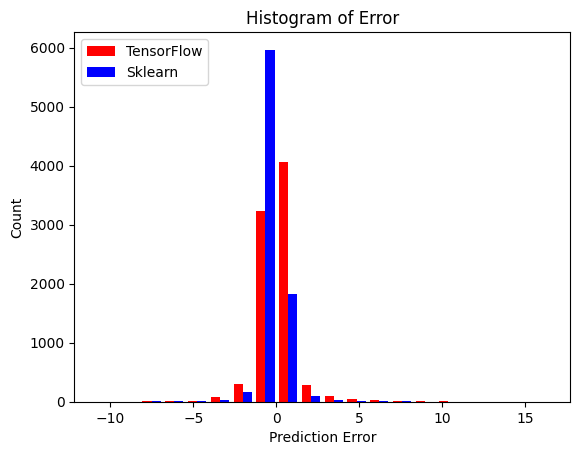
\includegraphics[width=3in]{histogram_patch}
    \captionof{figure}{Histogram of Error for Patch Antenna}
    \label{histogram_of_error_patch}
\end{Figure}

\begin{Figure}
    \centering
    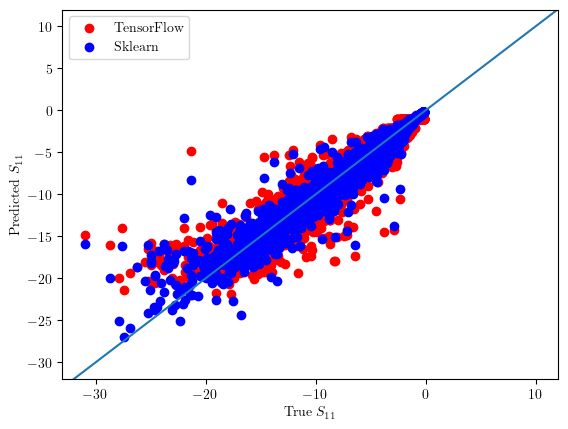
\includegraphics[width=3in]{actual_vs_predicted_s11_patch}
    \captionof{figure}{Actual vs Predicted $S_{11}$ for Patch Antenna}
    \label{actual_vs_predicted_s11_patch}
\end{Figure}

Figures~\ref{histogram_of_error_leaky_wave} and~\ref{actual_vs_predicted_s11_leaky_wave} show how the results for the leaky wave antenna are similar to those of the patch antenna. The leaky wave antenna was trained on significantly fewer geometries, which is reflected by the poorer overall performance of both the DNN model and the Scikit-learn model. Similarly to with the patch antenna, both figures prove that the Scikit-learn model makes $S_{11}$ predictions with higher accuracy than the DNN model.

\begin{Figure}
    \centering
    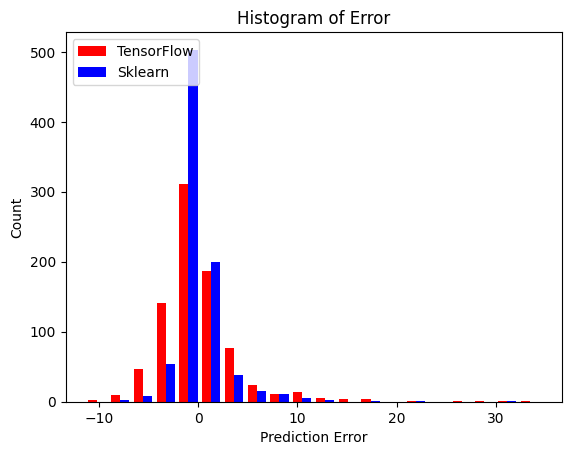
\includegraphics[width=3in]{histogram_leaky_wave}
    \captionof{figure}{Histogram of Error for Leaky Wave Antenna}
    \label{histogram_of_error_leaky_wave}
\end{Figure}

\begin{Figure}
    \centering
    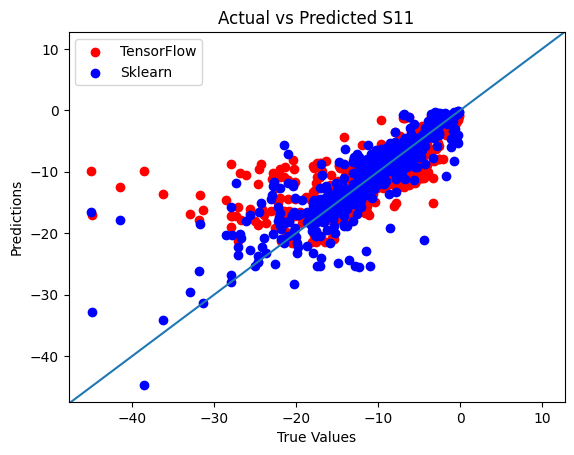
\includegraphics[width=3in]{actual_vs_predicted_s11_leaky_wave}
    \captionof{figure}{Actual vs Predicted $S_{11}$ for Leaky Wave Antenna}
    \label{actual_vs_predicted_s11_leaky_wave}
\end{Figure}

\subsection{Testing with Unseen Geometries}
The chosen model was given a set of six random geometries from the patch antenna that had never been seen before by either the training set or testing set. These geometries were part of the permutations that were generated to create the dataset for optimal geometry searching. 

These unseen geometries were run through both the HFSS and the chosen machine learning model in order to obtain simulated and predicted $S_{11}$ values. This process was completed for the entire frequency range of the patch antenna. The results are shown in Figure~\ref{unseen_geometries_graph}, where each unseen geometry has its simulated $S_{11}$ values plotted alongside the predicted values for each frequency in the frequency range. This process was completed for both the patch antenna and the leaky wave antenna.

For the patch antenna, it's interesting to note how the prediction of the $S_{11}$ values of Geometry 2 was nearly identical to the simulated values. For Geometries 3, 4, and 6, both the predicted values and the simulated values had similar dips in the curves around 7GHz and 11GHz. However, the dips were shifted to slightly lower frequency ranges for the predicted values. Additionally, for all geometries tested, the predicted $S_{11}$ values appear to follow the same trend as the simulated values, but they never reach as far low as the simulated values go. 

\textlangle Write about unseen geometries for leaky wave here \textrangle


\begin{Figure}
    \centering
    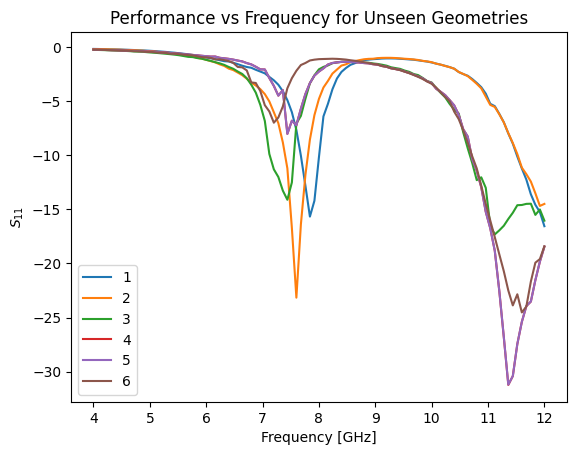
\includegraphics[width=3.25in]{unseen_geometries_freq_vs_seq}
    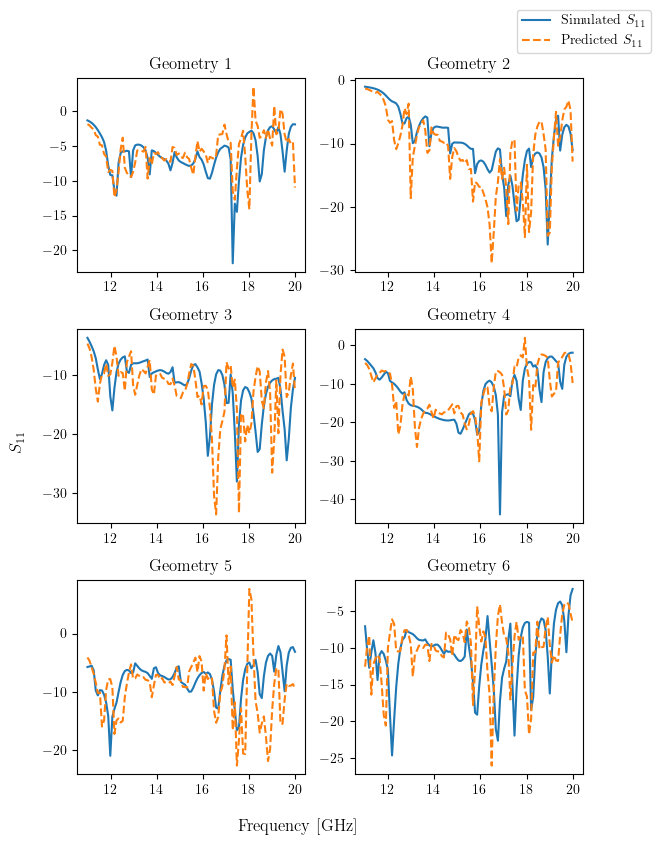
\includegraphics[width=3.25in]{unseen_geometries_freq_vs_seq_lw}
    \captionof{figure}{Simulated \& Predicted $S_{11}$ Values for Frequency Range of Unseen Geometries for Patch Antenna and Leaky Wave Antenna}
    \label{unseen_geometries_graph}
\end{Figure}


\subsection{Finding Optimal Geometry}
A graphical user interface (GUI) was implemented using Jupyter Widgets to allow for ease of exploring different types of geometries~\cite{interactive_Jupyter_widgets}. A user inputs a desired $S_{11}$ value and frequency range, and a graph showing predicted $S_{11}$ values for the frequency range will be plotted for the best performing geometries. This graph includes marker lines as a visual aid to show what value the $S_{11}$ predictions should be below and what frequency values the predictions should be between. The GUI allows the user to interactively explore which geometric parameters lead to a specified performance, where before this was a manual and timely process.  


An example of an input and the corresponding graph that is generated is shown in Figure~\ref{gui}. The specified $S_{11}$ value of -25dB is represented by the dotted horizontal blue line, and the selected frequency range between 12.81GHz and 13.03GHz is represented by the two dotted vertical green lines. All of the 4 geometries that are found have predicted $S_{11}$ values within these constraints. Table~\ref{gui_geometries} shows the 4 optimal geometries that are represented in Figure~\ref{gui}. The geometries that are best for this criteria have a $feed\_l$ of 3.75mm and a $patch\_l$ of 4.0mm. The rest of the geometric parameters vary. 

\begin{Figure}
    \centering
    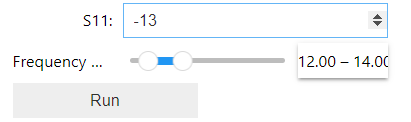
\includegraphics[width=2in]{gui_input}
    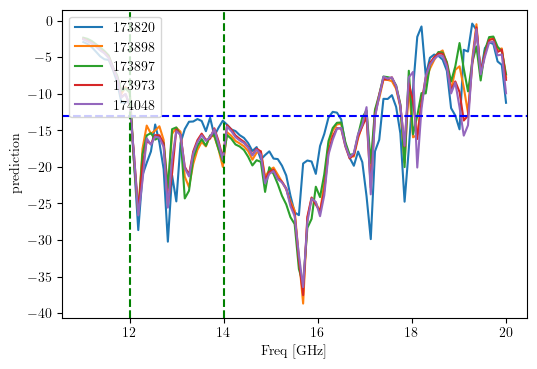
\includegraphics[width=3in]{gui_graph}
    \captionof{figure}{GUI Input and Predicted $S_{11}$ vs Frequency for Optimal Geometries}
    \label{gui}
\end{Figure}

\begin{table}[h]
\caption{Geometries Generated from GUI}
\begin{center}
\begin{tabular}{ 
|p{1.75cm}|p{1cm}|p{1cm}|p{1cm}|p{1cm}|p{1cm}|}
    \hline
    ID & 17505219 & 17528247 & 17528348 & 17535822 & 17543397 \\
    \hline
    cpw\_in [mm] & 2.00 & 2.00 & 2.00 & 2.00 & 2.00 \\
    \hline
    feed\_l [mm] & 4.00 & 4.00 & 4.00 & 4.00 & 4.00 \\
    \hline
    patch\_l [mm] & 3.50 & 3.50 & 3.50 & 3.50 & 3.50 \\
    \hline
    cpw\_g [mm] & 0.18 & 0.18 & 0.18 & 0.18 & 0.18 \\
    \hline
    Feed\_W [mm] & 1.00 & 1.25 & 1.25 & 1.50 & 1.75 \\
    \hline
    ground\_w [mm] & 1.50 & 1.50 & 1.50 & 1.50 & 1.50 \\
    \hline
    patch\_ground\_w [mm] & 1.25 & 1.50 & 1.50 & 1.50 & 1.50 \\
    \hline
    patch\_w [mm] & 4.75 & 4.75 & 4.50 & 4.75 & 4.75 \\
    \hline
\end{tabular}
\end{center}
\label{gui_geometries}
\end{table} 


\subsection{SHAP}
In order to feasibly use SHAP with the patch antenna dataset, a random sample of 5,000 points was used. This sample consisted of all of the geometric parameters and the frequency, and accurately captures characteristics and trends present of the entire dataset. The best performing model, which was XGBRegressor, was used with scaled data in order to interface with the SHAP primary explainer. 

    
\begin{Figure}
\centering
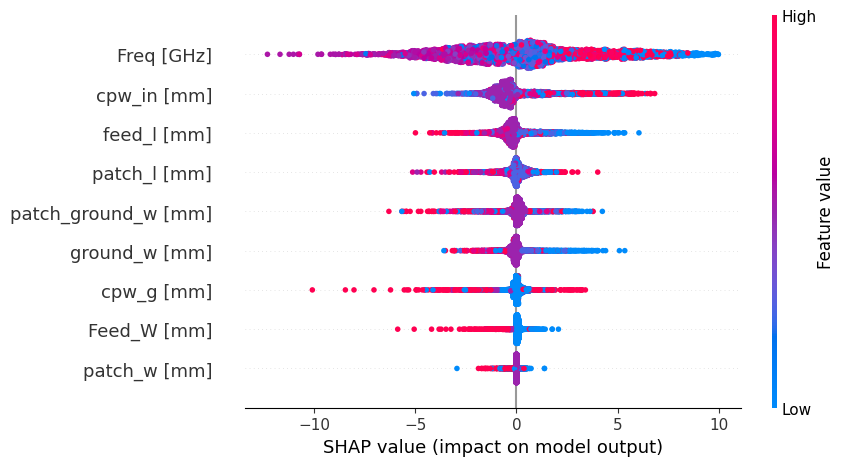
\includegraphics[width=3in]{shap_beeswarm}
\captionof{figure}{Beeswarm Plot of Features Impacting Predictions}
\label{shap_beeswarm}
\end{Figure}

Figure~\ref{shap_beeswarm} is a SHAP beeswarm plot, which is used to demonstrate the impact that each feature had on the predictions made by the model overall. The figure shows how frequency had a significantly higher impact on $S_{11}$ predictions than any geometric feature, and this makes sense when considering that every unique geometry configuration has $S_{11}$ predictions that generally follow the same pattern across the frequency range. All of the other geometric parameters appear to have similar impacts on the predictions being made. $feed\_l$, $ground\_l$, and $Feed\_W$ all very consistently had higher values of these features causing lower predictions to be made, and lower values causing higher predictions. The opposite was true for $cpw\_in$, with most higher feature values causing higher $S_{11}$ predictions. $cpw\_g$ was a bit different than the rest of the features, where high feature values caused both high and low predictions, but lower feature values caused the prediction to stay relatively the same. None of the other features had this strong of a correlation, and appeared to be more randomly distributed. 

\section{Conclusion}
Applying a machine learning algorithm as an aid in the process of optimizing antenna geometric parameters with EM simulations greatly reduces the amount of time and computational power required. Training a model on a small set of data obtained from running simulation software allows the model to fit to the trend of data. Large amounts of additional data can then be generated within the bounds of the existing data, and performance predictions can be made for this generated data with a high accuracy. The most optimal geometries can be returned for specified performance values and frequency ranges, making it unnecessary to run use a trial-and-error process to find these geometries by running simulations. Open-source ML explainability libraries can then be applied to the model and data to allow for further analysis of the contribution each geometric feature makes to the predictions. 


\bibliographystyle{IEEEtran}
\bibliography{refs}

\vfill

\end{document}